\documentclass[a4paper]{panl}
\usepackage{cite}
\usepackage{wrapfig}
\usepackage{graphicx}
\usepackage{amssymb}
\usepackage{amsfonts}
\usepackage{amsmath}
\usepackage{longtable}
\usepackage{rotating}
\usepackage{lscape}
\usepackage{epsfig}
\usepackage{multirow}
\usepackage{color}

\originalTeX
%\russianTeX
\begin{document}
% Journal sections (see http://pkp.jinr.ru/index.php/PEPAN_LETTERS/about/editorialPolicies#focusAndScope)
\issuearea{Physics of Elementary Particles and Atomic Nuclei}
% or in Russian
%\issuearea{ФИЗИКА ЭЛЕМЕНТАРНЫХ ЧАСТИЦ И АТОМНОГО ЯДРА. ТЕОРИЯ}

\title{Femtoscopy with identified charged particles for the NICA energy range}
\maketitle
\authors{P.\,Batyuk$^{~a,}$\footnote{E-mail: pavel.batyuk@jinr.ru}, 
L.\,Malinina$^{~a, b}$, K. Mikhaylov$^{~a, c}$, G. Nigmatkulov$^{~d}$}
\from{$^{a}$\, Joint Institute for Nuclear Research, Dubna, Russia}
\vspace{-3mm}
\from{$^{b}$\, Skobeltsyn Research Institute of Nuclear Physics, Moscow State University, Moscow, Russia}
\vspace{-3mm}
\from{$^{c}$\, The Institute for Theoretical and Experimental Physics, State Scientific Center of the Russian Federation, Moscow, Russia}
\vspace{-3mm}
\from{$^{d}$\, National Research Nuclear University MEPhI, Moscow, Russia}


\begin{abstract}
  The correlation femtoscopy allows one to measure the space-time characteristics of particle production processes
  due to the effects of quantum statistics (QS) and final state interactions (FSI).
  Femtoscopy at lower energies was intensively studied at AGS, SPS and in the Beam Energy Scan (BES) program at RHIC.
  In the work we discuss possibilities to observe a difference from the first-order phase transition expected, according 
  some theoretical predictions, at low energies and the crossover one, to be occurred at high energies, with the femtoscopy 
  observables using the hybrid model vHLLE+UrQMD.
  The possibilities to use kaon femtoscopy complementary to the usually used pion one are discussed.
\end{abstract}
\vspace*{6pt}

\noindent
PACS:

%% Figures to be inserted
\vspace{-6mm}
\label{sec:intro}
\section*{Motivation}

The well developed femtoscopy formalism is considered as a very powerful tool to be used for study of the space-time evolution 
occurred in course of heavy-ion collision. The NICA energy range ($\sqrt{s_{NN}} = 4 - 11$ GeV) with existing (BM@N) and future 
experiments (MPD, SPD) to be operated looks very promising.
In particular, it would allow one, due to a high planned level of luminosity, to extend the usually used set of pion femtoscopic 
observables to heavier particles to perform measurements with higher accuracy.     

An assumption that the nuclear matter undergoes the first-order phase transition, probably, to be occurred at the NICA energies 
motivated our studies. In~\cite{Rischke:1996em} it was shown that the first-order phase transition leads to a stalling of the expansion 
speed and increase of the emission duration, $\Delta \tau$. As a result, it leads to increasing of $R_{long}$ and $R_{out} / R_{side}$.
From experimental point of view, femtoscopy with charged identical pions performed within the BES program allowed one to observe 
maximum in the excitation function of $R_{out} / R_{side}$ distribution at around $\sqrt{s_{NN}}$ = 20 GeV~\cite{Adamczyk:2014mxp}. 
Its presence could be attributed to a possible expected change of nuclear matter equation of state (EoS) and type of phase transition.
At the same time, since the NICA energy range according to some theoretical predictions is a baryon dominated one, it allows one 
to do a search for change of the phase transition type by making use of femtoscopy tools, e.g. analysing behaviour of the observables.

To shed light on it, it sounds reasonably to perform a detailed feasibility study on it by use of modern
hybrid (``sandwich''-like) Monte Carlo generators. As a candidate to be used, we have taken the vHLLE+UrQMD model.
To be known for the model in detail the reader is referred to~\cite{Karpenko:2015xea}. The reasons caused our choice and to be mentioned 
here obligatory are related to a huge set of benefits available for our studies with the model. The first one is that the model was tuned 
with existing experimental data to be able to reproduce quantitatively well a set of bulk observables
(yields, $p_{t}$ and rapidity spectra). The second one is that the model has an option to change EoS when doing simulations. 
It supports two types of EoS to be used. To be familiar with them, one is addressed to~\cite{Steinheimer:2010ib, Kolb:2000sd}. 
The last but not least mentioned here is that the model demonstrates, as shown in Fig.~\ref{fig01}, a dependence of the average pion 
creation time at the particlization surface and the last interactions on collision energy as a function of the EoS used
in course of simulations. The calculations involving the first-order phase transition are denoted by 1PT, meanwhile those ones corresponded 
to the crossover EoS are denoted by XPT.
The dependence looks apparently weak and the hadronic cascade smears the visible difference, but, nevertheless, it remains thus 
allowing one to use the model for investigating observables which are sensitive to the EoS scenario assumed. 

\begin{figure}[t]
\begin{center}
  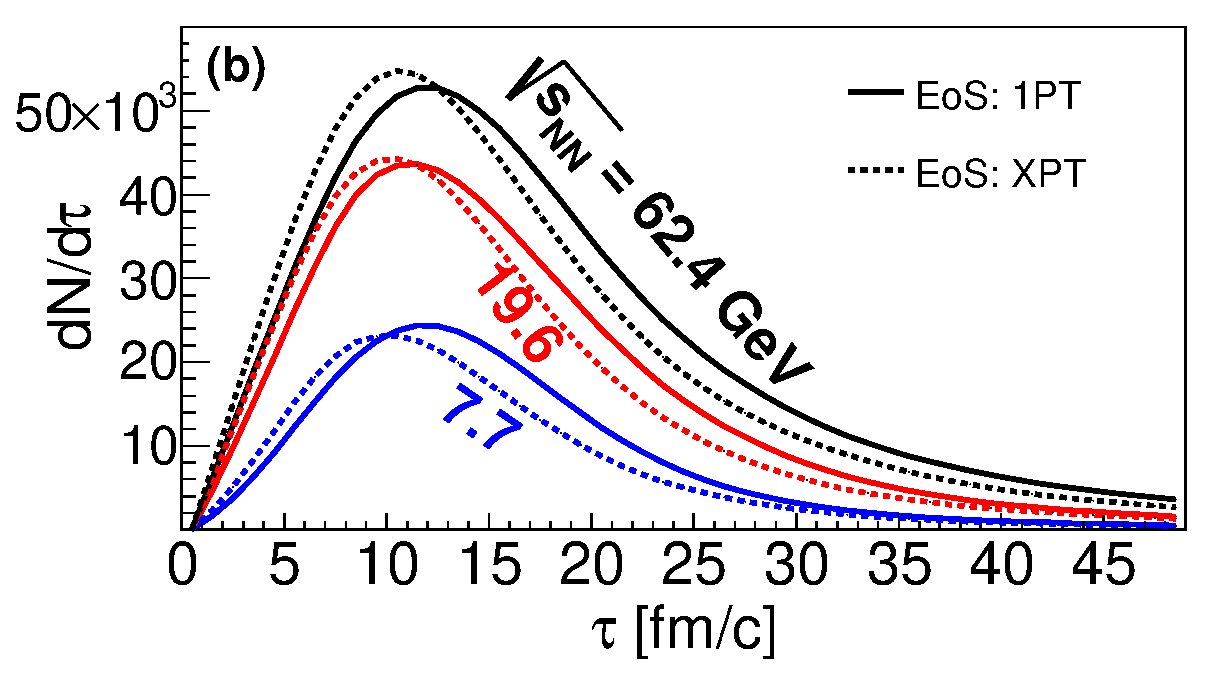
\includegraphics[width=60mm]{fig1b.eps}
  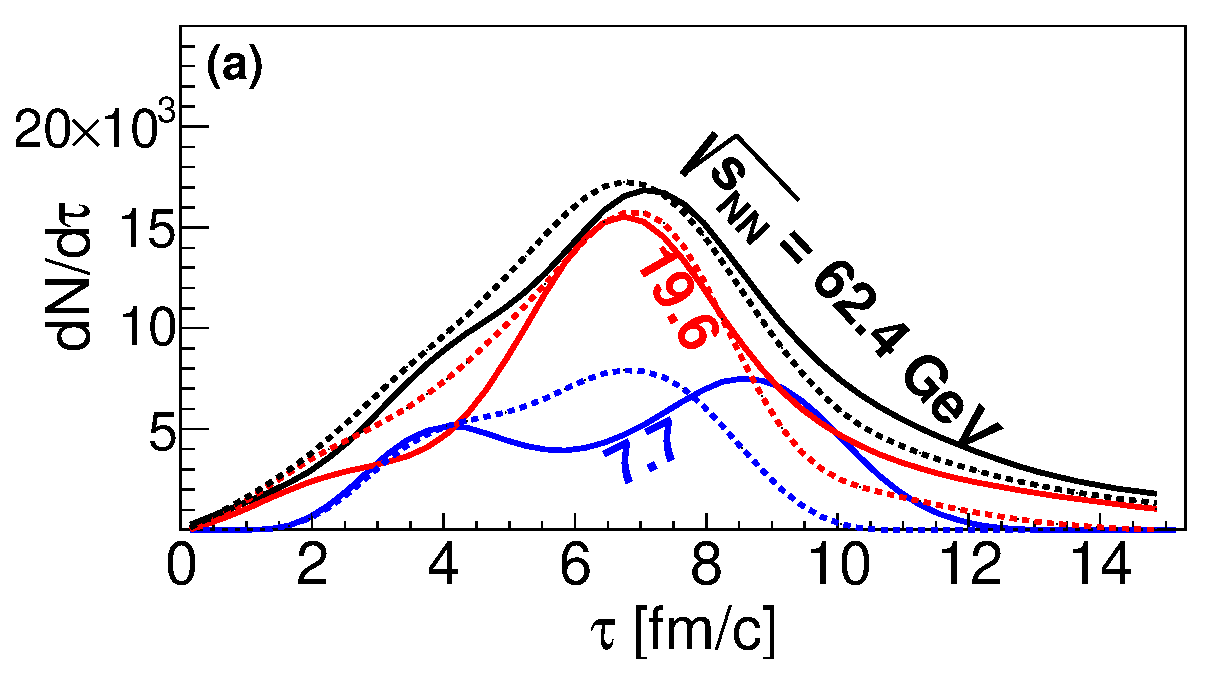
\includegraphics[width=60mm]{fig1a.eps}
\vspace{-3mm}
\caption{Pion emission times at the particlization surface (a) and the last interactions (b) in the center-of-mass system of colliding gold nuclei at different values of $\sqrt{s_{NN}}$.}
\end{center}
\labelf{fig01}
\vspace{-5mm}
\end{figure}

\label{sec:Results_and_discussion}
  \section*{Results and discussion}
  The current paper is considered as a continuation of our studies already done with the model. The previous studies aimed to extract pion 
  femtoscopy radii from three-dimensional   correlation functions are considered extensively in~\cite{Batyuk:2017smw}.
  We extracted the femtoscopic radii, $R_{out, side, long}$, the difference, $R^{2}_{out} - R^{2}_{side}$, and the ratio, $R_{out} / R_{side}$, 
  to be compared with existing experimental data on pion femtoscopy obtained from the BES program~\cite{Adamczyk:2014mxp} as a function 
  of collision energy. 
  The used parametrization of correlation function is a standard one described in~\cite{Pratt:1986cc, Bertsch:1988db}.
  \begin{figure}[t]
    \begin{center}
      \includegraphics[width=115mm]{fig2.eps}
      \vspace{-3mm}
      \caption{Comparison of the model pion femtoscopy radii with those obtained from the BES program at
        $\sqrt{s_{NN}}$ = 7.7 ((a) - (d)), 11.5 ((e) - (h)), 19.6 ((i) - (l)), 27 ((m) - (p)), 39 ((q) - (t)), 62.4 ((u) -(x)) GeV.
        Open squares represent experimental data. Green and red triangles correspond to the 1PT EoS and XPT EoS respectively.}
    \end{center}
    \labelf{fig02}
    \vspace{-5mm}
  \end{figure}

  One can see, as shown in Fig.~\ref{fig02}, that the model reasonably describes the $m_{T}$-dependence of radii for all available 
  energies with both scenarios of the EoS used.
  The radii demonstrate different trends in the out, side and long directions. $R_{side}$ seems to be almost the same for both scenarios.
  $R_{out}$ has a tendency to be larger of order of 0.5~fm when using the 1PT EoS.
  A longer lifetime of the fluid phase in the 1PT EoS leads to bigger values of $R_{long}$ if comparing with the XPT EoS.

  \begin{figure}[t]
    \begin{center}
      \includegraphics[width=70mm]{fig3.png}
      \vspace{-3mm}
      \caption{Ratio of femtoscopic radii calculated for the two available scenarios of EoS.}
    \end{center}
    \labelf{fig03}
    \vspace{-5mm}
  \end{figure}
  
  
  Results of another test performed regarding to the sensitivity of femtoscopic observables to the EoS used for simulation are shown in Fig.~\ref{fig03}.
  It represents a ratio of femtoscopic radii extracted from simulations done with the 1PT EoS (nominator) and those ones with the XPT EoS (denominator).
  Seen that $R_{side}$ coincides for both scenarios, meanwhile $R_{out}$ and $R_{long}$ are larger for the 1PT EoS and demonstrate a strong $k_{T}$-dependence.
  It confirms the well known fact that for the 1PT EoS the radial flow developed in the pre-hydro phase of collision is weaker than for the XPT EoS thus emphasizing a strong role
  of radial flow effects.
    
  As already told, all we did in~\cite{Batyuk:2017smw} is related to pions, thus a logical continuation of the studies mentioned above includes its expansion to charged identical kaons.
  
 \begin{figure}[t]
    \begin{center}
      \includegraphics[width=100mm]{fig4a.png}
      \includegraphics[width=100mm]{fig4b.png}
      \vspace{-3mm}
      \caption{Projections of three-dimensional correlation functions for pions ((a) - (c)) and \newline kaons~((d) - (f)) on out, side and long directions.
      The calculations made at $\sqrt{s_{NN}}$ = 11.5 GeV.}
    \end{center}
    \labelf{fig04}
    \vspace{-5mm}
  \end{figure}

 Results of the first step of this analysis, mainly related to study on how the projections of kaon three-dimensional correlation functions on out, side and long directions look like,
 are shown in Fig.~\ref{fig04} ((d) - (f)) in comparison with those corresponding to the pion ones (upper row of Fig.~\ref{fig04}). The parametrization of correlation function used to fit
 the Gaussian radii is given in~\cite{Batyuk:2017smw}, where one could be referred to.
 The kaon projections on all directions seem to be more Gaussian if comparing with pions. The projections extracted from the simulations assuming the XPT EoS scenario are visibly wider than
 for the 1PT EoS. The effect observed is more significant for kaons.   

\begin{figure}[t]
  \begin{center}
     \includegraphics[width=100mm]{fig5a.pdf}
     \includegraphics[width=100mm]{fig5b.pdf}
\vspace{-3mm}
\caption{Comparison of the model pion and kaon femtoscopy radii for two energies $\sqrt{s_{NN}}$ = 7.7, 11.5 GeV close to the NICA energy range
  with pion data got from the BES program.}
\end{center}
\labelf{fig05}
\vspace{-5mm}
\end{figure}

In Fig.~\ref{fig05} the $m_{T}$-dependence of the extracted kaon radii is shown for two energies in the NICA energy range and both possible scenarios of EoS used for simulations.
The model calculations are compared with existing data for pions got from the BES program.
One can see that the general behaviour of the kaon and pion radii from the model is very similar. For both cases the radii and the $R_{out} / R_{side}$ ratio corresponding
to the 1PT EoS are larger than those ones for the XPT EoS. Despite the almost similar general behaviour, it is seen that
the kaon $R_{out}$ has a tendency to diverge for the two types of EoS with increase of $m_{T}$. Probably, it can be attributed to the weak radial flow developed in the pre-hydro phase of
collision, but it is just an assumption since it has not been investigated yet in detail right now and is planned to be done in the future. 
  
\label{sec:Acknowledgements}
\section*{Acknowledgements}
The work has been supported by the grant of Russian Foundation for Basic Research ({\bf 18-02-40044}) and also partially supported
by the National Research Nuclear University MEPhI in the framework of the Russian Academic Excellence Project 
(contract No. 02.a03.21.0005, 27.08.2013).
The authors would like to thank Yu.~Sinyukov, Yu.~Karpenko and L.~Rednick\'{y} for their great contribution to the work and 
possibilities to have fruitful discussions aimed at doing the work clearer and better.
Also, we thank N. Kutovskiy and his team~\cite{jinrCloud} for using the well equipped JINR cloud infrastructure to perform 
the calculations presented in the paper.

\begin{thebibliography}{1}
\def\selectlanguageifdefined#1{
\expandafter\ifx\csname date#1\endcsname\relax
\else\selectlanguage{#1}\fi}
\providecommand*{\href}[2]{{\small #2}}
\providecommand*{\url}[1]{{\small #1}}
\providecommand*{\BibUrl}[1]{\url{#1}}
\providecommand{\BibAnnote}[1]{}
\providecommand*{\BibEmph}[1]{\emph{#1}}
\ProvideTextCommandDefault{\cyrdash}{\hbox to.8em{--\hss--}}
\providecommand*{\BibDash}{\ifdim\lastskip>0pt\unskip\nobreak\hskip.2em\fi
  \cyrdash\hskip.2em\ignorespaces}

\bibitem{Rischke:1996em} 
  D.~H.~Rischke and M.~Gyulassy,
  %``The Time delay signature of quark - gluon plasma formation in relativistic nuclear collisions,''
  Nucl.\ Phys.\ A {\bf 608}, 479 (1996)
  doi:10.1016/0375-9474(96)00259-X
  [nucl-th/9606039].
  %%CITATION = doi:10.1016/0375-9474(96)00259-X;%%
  %294 citations counted in INSPIRE as of 15 Aug 2019

\bibitem{Adamczyk:2014mxp} 
  L.~Adamczyk {\it et al.} [STAR Collaboration],
  %``Beam-energy-dependent two-pion interferometry and the freeze-out eccentricity of pions measured in heavy ion collisions at the STAR detector,''
  Phys.\ Rev.\ C {\bf 92}, no. 1, 014904 (2015)
  doi:10.1103/PhysRevC.92.014904
  [arXiv:1403.4972 [nucl-ex]].
  %%CITATION = doi:10.1103/PhysRevC.92.014904;%%
  %60 citations counted in INSPIRE as of 15 Aug 2019

\bibitem{Karpenko:2015xea} 
  I.~A.~Karpenko, P.~Huovinen, H.~Petersen and M.~Bleicher,
  %``Estimation of the shear viscosity at finite net-baryon density from $A+A$ collision data at $\sqrt{s_\mathrm{NN}} = 7.7-200$ GeV,''
  Phys.\ Rev.\ C {\bf 91}, no. 6, 064901 (2015)
  doi:10.1103/PhysRevC.91.064901
  [arXiv:1502.01978 [nucl-th]].
  %%CITATION = doi:10.1103/PhysRevC.91.064901;%%
  %70 citations counted in INSPIRE as of 15 Aug 2019

\bibitem{Steinheimer:2010ib} 
  J.~Steinheimer, S.~Schramm and H.~Stocker,
  %``An Effective chiral Hadron-Quark Equation of State,''
  J.\ Phys.\ G {\bf 38}, 035001 (2011)
  doi:10.1088/0954-3899/38/3/035001
  [arXiv:1009.5239 [hep-ph]].
  %%CITATION = doi:10.1088/0954-3899/38/3/035001;%%
  %68 citations counted in INSPIRE as of 15 Aug 2019

\bibitem{Kolb:2000sd} 
  P.~F.~Kolb, J.~Sollfrank and U.~W.~Heinz,
  %``Anisotropic transverse flow and the quark hadron phase transition,''
  Phys.\ Rev.\ C {\bf 62}, 054909 (2000)
  doi:10.1103/PhysRevC.62.054909
  [hep-ph/0006129].
  %%CITATION = doi:10.1103/PhysRevC.62.054909;%%
  %562 citations counted in INSPIRE as of 15 Aug 2019

\bibitem{Batyuk:2017smw} 
  P.~Batyuk, I.~Karpenko, R.~Lednicky, L.~Malinina, K.~Mikhaylov, O.~Rogachevsky and D.~Wielanek,
  %``Correlation femtoscopy study at energies available at the JINR Nuclotron-based Ion Collider fAcility and the BNL Relativistic Heavy Ion Collider within a viscous hydrodynamic plus cascade model,''
  Phys.\ Rev.\ C {\bf 96}, no. 2, 024911 (2017)
  doi:10.1103/PhysRevC.96.024911
  [arXiv:1703.09628 [nucl-th]].
  %%CITATION = doi:10.1103/PhysRevC.96.024911;%%
  %2 citations counted in INSPIRE as of 15 Aug 2019

\bibitem{Pratt:1986cc} 
  S.~Pratt,
  %``Pion Interferometry of Quark-Gluon Plasma,''
  Phys.\ Rev.\ D {\bf 33}, 1314 (1986).
  doi:10.1103/PhysRevD.33.1314
  %%CITATION = doi:10.1103/PhysRevD.33.1314;%%
  %417 citations counted in INSPIRE as of 15 Aug 2019

\bibitem{Bertsch:1988db} 
  G.~Bertsch, M.~Gong and M.~Tohyama,
  %``Pion Interferometry in Ultrarelativistic Heavy Ion Collisions,''
  Phys.\ Rev.\ C {\bf 37}, 1896 (1988).
  doi:10.1103/PhysRevC.37.1896
  %%CITATION = doi:10.1103/PhysRevC.37.1896;%%
  %288 citations counted in INSPIRE as of 15 Aug 2019
  

\bibitem{jinrCloud} 
  A.~V.~Baranov, N.~A.~Balashov, N.~A.~Kutovskiy and R.~N.~Semenov,
  %``JINR cloud infrastructure evolution,''
  Phys.\ Part.\ Nucl.\ Lett.\  {\bf 13}, no. 5, 672 (2016).
  doi:10.1134/S1547477116050071
  %%CITATION = doi:10.1134/S1547477116050071;%%
  %2 citations counted in INSPIRE as of 15 Aug 2019
\end{thebibliography}
\end{document}
